\chapter{Lesson 5}
\section{Overview}
In lesson one of this special feature on learning the guitar, we were introduced to the parts of the guitar, learned to tune the instrument, learned a chromatic scale, and learned Gmajor, Cmajor, and Dmajor chords. Guitar lesson two taught us to play Eminor, Aminor, and Dminor chords, an E phrygian scale, a few basic strumming patterns, and the names of the open strings. In guitar lesson three, we learned how to play a blues scale, Emajor, Amajor, and Fmajor chords, and a new strumming pattern. Lesson four introduced us to power chords, basic note names on the sixth and fifth string, and new strumming patterns. If you are not familiar with any of these concepts, it is advised that you revisit these lessons before proceeding. 

\subsection{What You'll Learn in Lesson Five}

Get ready for a real challenge this week... lesson five will introduce a whole new type of chord that you'll use a lot in the future, the "barre chord". We'll also complete our learning of the note names on the sixth and fifth string, learn a blues shuffle and several guitar leads, as well as learn a bunch of new songs.

Are you ready? Good, let's start guitar lesson five. 

\section{Sharps and Flats}
In guitar lesson four, we learned the names of the notes on the sixth and fifth string (you'll want to review them first if you're unsure of them). While that lesson was designed to teach you the basic note names, it did not tell you all you need to know as a guitarist. The following lesson will fill in the gaps lesson four intentionally avoided.

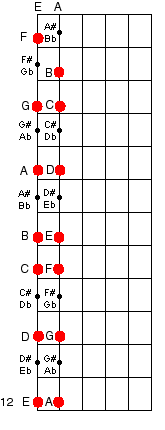
\includegraphics{partfive/fretboard_full.png}
If you've absorbed the material in lesson four, you'll know the names of all the notes in red on the diagram to the left. What you won't recognize is the names of the notes in between these red dots.

Let's begin by examining two new terms... "sharp" - which is written like this: \# , and "flat" - which is written like this: b . Essentially, the term sharp means a note is raised a note by one fret (a "semitone"), while flat means a note is lowered by one fret (a "semitone").

Upon studying the diagram to the left, you'll notice each "in-between" note has two alternate names: one being a letter name followed by a sharp sign, and the other being a letter name followed by a flat sign. To explain this, we'll name the note on the second fret of the sixth string. The note is one fret above the note F on the first fret, so we will refer to the note as an F sharp(F\#). Alternately, the same note is also one fret below the note G on the third fret, so it can also be referred to as G flat(Gb). You'll see this note referred to as either F\# or Gb (for theoretical reasons that don't concern us now), so you must be aware that they are the exact same note. This same principle holds true for all other notes on the fretboard. 

\subsection{Things to remember}
\begin{itemize}
\item "Sharp" is notated as \#
\item "Flat" is notated as b
\item If a letter name is followed by a sharp(\#), the note is one fret higher than the fret you'd normally play that letter name on. Example: you'd play G on the third fret, sixth string. You'd play G\# on the fourth fret sixth string.
\item If a letter name is followed by a flat(b), the note is one fret lower than the fret you'd normally play that letter name on. Example: you'd play D on the tenth fret, sixth string. You'd play Db on the ninth fret sixth string.
\item F\# = Gb, G\# = Ab, A\# = Bb, C\# = Db, D\# = Eb
\item The note name on the 12th fret of any string is always the same as the open string.
\item Memorize the open string name, and several more note names and locations on both the sixth and fifth string. This will make finding all other notes much quicker. 
\end{itemize}

\section{12 Bar Blues}
Learning the blues is an essential step in becoming a well-rounded guitarist. Since the basic blues is so simple, many guitarists will use it as a common ground - a means of playing with others who they've never played with before. Consider this: a 50 year old man, and a 14 year old teenager are trying to play guitar together. Chances are, they're not going to know many of the same songs. This is when knowing a simple blues will come in handy... one guitarist can play the chords, and the other can either sing, or play guitar solos over those chords. And then, they can trade off, to let them both have a turn playing lead guitar.

The following provides instructions for learning a 12-bar blues in the key of A. There is a very simple intro and outro which have been included, which might take a little practice to play quickly, but shouldn't be too difficult. For the sake of simplicity, the following is presented in a very basic, almost "hokey" style. Learn it as is, and we'll vary the style in upcoming lessons, to make the blues sound a little more interesting. 

\subsection{The Intro}
This is a blues intro at it's most basic.. just a few chords, and a few single notes, which will lead nicely into the main part of the song. 

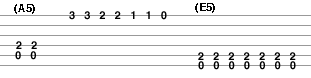
\includegraphics{partfive/shuffleintrotab.png}

\subsection{The Outro}
This is a basic guitar part that will wrap up the song, the last time you play it. It's not very long, and shouldn't be too tough to learn. 

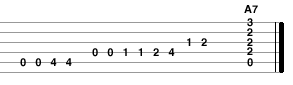
\includegraphics{partfive/shuffleoutrotab.png}

\subsection{The 12 Bar Blues}
This is the main part of the song. The song starts with a simple intro (not shown below), then continues for 12 bars, then repeats (without repeating the intro). The last time the song is played, the last two bars are replaced by the outro. 

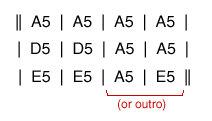
\includegraphics{partfive/shufflebluesform.png}

The above gives the general breakdown of the twelve bar blues, and you'll need to memorize it. Chances are, though, when you hear it played, it will sound logical, and shouldn't be at all hard to memorize.
Although the above diagram shows us generally which chords we will play in each bar, we are going to play something a little more complex than just A5 for four bars, D5 for two bars, etc. To see exactly what you'll play for each bar, study the following: 

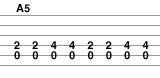
\includegraphics{partfive/shufflea5tab.png}

For each bar of A5, you'll play the above tablature. Play the note on the second fret with your first finger, and the note on the fourth fret with your third finger. 

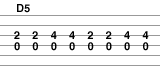
\includegraphics{partfive/shuffled5tab.png}

For each bar of D5, you'll play the above tablature. Play the note on the second fret with your first finger, and the note on the fourth fret with your third finger. 

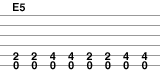
\includegraphics{partfive/shufflee5tab.png}

For each bar of E5, you'll play the above tablature. Play the note on the second fret with your first finger, and the note on the fourth fret with your third finger.

If you listen to the recording, you'll notice there's one small variation not included so far. It is this: the first time through the 12 bar blues, on the 12th bar, we play a different pattern on the E5 chord. This is often done at the end of each 12 bars, because it gives the listener and the band a solid way of knowing that we're at the end of the song form, and we're going back to the beginning again. Here is how you play this very simple pattern: 

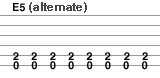
\includegraphics{partfive/shufflee5alternate.png}

And, that's it! Looking at all the above instructions, you're probably going to feel overwhelmed. Pick up your guitar, and try playing through it all... it's actually quite simple, and rather easy to memorize. 

\subsection{Things to try}
\begin{itemize}
\item Loop the 12 bar blues without an intro, and without the outro. Keep repeating the 12 bar form, until you've memorized it.
\item Try playing the intro and outro, along with the song, WITHOUT losing the timing.
\item Play along to the recorded examples.
\item Try playing an A blues scale over the recorded example. This is something we're going to examine further in the future.
\item Be sure you're not hitting open strings that you shouldn't be playing. 
\end{itemize}

\section{The B Minor Chord}
Here's where we take the next big step in our progress as a guitarist... learning about a shape of chord referred to as a "barre chord". The technique of playing barre chords is one which we have utilized when playing the F major chord - using one finger to hold down more than one note.

\subsection{The B minor shape}
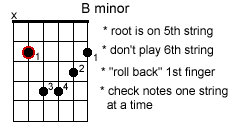
\includegraphics{partfive/bminor.png}

We're going to put your first finger to work on this chord. Your first finger has the job of covering the second fret, from the fifth to first strings (we don't play the sixth string). Next, put your third finger on the fourth fret of the fourth string. Then, add your fourth pinky finger to the fourth fret of the third string. Lastly, place your second finger on the third fret of the second string. Got it? Now, strum the chord, and try not to get upset when most of the notes don't ring clearly.

This is a tough chord at first, no doubt about it! You're going to have to have patience, it WILL sound good soon, but it's going to take some work. Here are some tips that will help you:
\begin{itemize}
\item Very slightly bend your first finger. A straight and rigid finger is not what we're looking for.
\item Roll the finger back slightly, so that more of the side of the index finger closest to the thumb is in contact with the strings.
\item Try slightly pulling the body of the guitar towards your body, using the arm of your picking hand. Also gently pull the neck towards you with your fretting hand. This makes fretting barre chords somewhat easier. 
\end{itemize}

\subsection{Movable chord}
One of the greatest things about the B minor chord shape is that it is a "movable chord". This means that, unlike the chords we've learned so far, we can slide the same shape around to different frets to create different minor chords. The note we're interested in is the note on the fifth string. Whatever note your finger is playing on the fifth string is the type of minor chord it is. If you were to slide the chord up the neck, so that your first finger was at the fifth fret, you'd be playing a D minor chord, since the note on the fifth fret of the fifth string is D. THIS is why learning the note names on the sixth and fifth strings are so important. We'll be getting into different movable chords in the next lesson. 

\subsection{Things to try}
\begin{itemize}
\item Hold the shape of the B minor chord, and play strings one at a time. Correct any notes that aren't ringing clearly.
\item Try moving from other chords to a B minor chord, then back to other chords. This will be a slow and difficult process at first. Keep trying!
\item Try playing different minor chords by moving the B minor shape around to different frets (eg. try playing C\# minor, F minor, G minor, Bb minor, etc.)
\item Do NOT play the sixth string when playing a B minor chord. Pay careful attention to this. 
\end{itemize}

\section{Scale Review}
The blues scale plays a big part in rock in pop music, both in the solos of guitarists, and often within the songs themselves. In lesson three, we learned the basics of the blues scale. Now, we'll review the scale, and explore it a little bit further. 

\subsection{The Blues Scale}
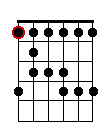
\includegraphics{partfive/bluesscale2.png}

If you're having trouble remembering exactly how to play the blues scale, have a look at the diagram on the left. Truthfully, it's one of the easier scales you'll learn.. probably because your first finger starts on the same fret of each string. Play the scale forwards and backwards several times.

What fret you start this scale at depends on which scale you'd like to play.. like the B minor chord we learned in this lesson, the blues scale is "movable". What type of blues scale you're playing depends on which fret you start at. If you start the scale with your first finger on the fifth fret of the sixth string (the note A), you're playing an "A blues scale". If you start the scale with your first finger on the eighth fret of the sixth string, you're playing a "C blues scale". 

\subsection{Uses of Blues Scale}
If you're interested in learning to play guitar solos, you'll want to spend a whole lot of time with the blues scale. Many pop, rock, and blues guitarists use the blues scale almost exclusively in their solos. The basic premise is this: a guitarist will play a series of notes from the blues scale, which sound good together. Learning to do this well takes experimentation and practice, but it gets easier.

Many songwriters use parts of the blues scale as the foundation for their songs. Led Zeppelin did this often: in the song Heartbreaker for example, the blues scale is used extensively in the main "guitar riff". Eric Clapton used the blues scale too, for the riff in Cream's Sunshine of Your Love. 

\subsection{Things to try}
\begin{itemize}
\item Play the scale forwards and backwards. Try starting in the middle of the scale, and finishing it, going forwards, and backwards. In short... memorize it well!
\item Experiment with playing various notes from the A blues scale along with this week's blues shuffle (click to hear audio)
\item If you have an interest in learning more about soloing, study the older archived lesson Learning to Improvise.
\item Play around with the notes in the blues scale, and see if you can't come up with a cool "guitar riff" that could be the basis of a song. 
\end{itemize}

\section{Learning Songs}
Since we've now covered all the basic open chords, plus power chords, and now the B minor chord, there are a countless number of songs to tackle. This week's songs will be focus on both open and power chords. 

Like a Rolling Stone - performed by Bob Dylan
NOTES: Try strumming this one as Down, Down, Down, Down up. Some rather quick chord changes in this song will keep you on your toes!
Wonderful Tonight - performed by Eric Clapton
NOTES: Here's a nice easy one. Strum chords 8x downwards each, with a few exceptions (use your ears to tell you which ones).Instead of D/F\#, play Dmajor. If you're brave, you can try the lead guitar part (it's not that hard).
Hotel California - performed by The Eagles
NOTES: okay this one is tough... since it uses a Bminor, and many other chords. There is also a new chord: F\#, which you'll play like this: play an Fmajor chord, and slide your fingers up one fret (so your first finger is barring the first and second strings, second fret).. only play strings four through one for this chord. When you see Bm7, play Bminor. Good luck!
Otherside - performed by The Red Hot Chili Peppers
NOTES: This song is surprisingly easy. Learn the opening single note riff, and the chords (don't worry about the notes below the chords for now). Strum chords: down, down up, up down up. 

\section{Practice Schedule}
Realistically, in order to play the B minor chord properly, you're going to have to invest some time in practicing. Here is a routine I would suggest, in order to keep your progress moving smoothly.
\begin{itemize}
\item Make sure your guitar is in tune (review how to tune).
\item Warm up by playing the blues scale, forwards and backwards, several times. Play slowly, use alternate picking, and make sure each note rings clearly.
\item Play through all chords you know, including the open chords, power chords, and the B minor chord. Be sure you know the name and shape for each chord.
\item Spend time reviewing the note names on the sixth and fifth string. Memorizing these notes is essential. Start by memorizing a few notes on each string.
\item Review all strumming patterns we've covered. We've learned patterns in lesson two, lesson three, and lesson four. Try switching from chord to chord while using these patterns.
\item Review the F major chord. It might not sound perfect yet, but chances are, if you've been practicing it, it's getting better and better. Keep it up.
\item Try to play all of the songs above. Don't get frustrated if a song is too tough for you. Take a deep breath, and try some more. If you're feeling overwhelmed, move to an easier song, or try songs from previous lessons. 
\end{itemize}
As we continue to learn more and more material, it becomes easy to overlook the techniques we learned during earlier lessons. They are all still important, so it is advisable to keep going over older lessons, and be sure you're not forgetting anything. There is a strong human tendency to only practice things which we are already quite good at. You'll need to overcome this, and force yourself to practice the things you are weakest at doing.

If you're feeling confident with everything we've learned so far, I suggest trying to find a few songs you're interested in, and learn them on your own. You can use the guitar tab area of the site to hunt down the music that you'd enjoy learning the most. Try memorizing some of these songs, rather than always looking at the music to play them.

In lesson six, we'll learn more strumming patterns, a few 7th chords, another barre chord, new songs, and much more. Have fun until then, and keep practicing! 

